\section{Sequential Locking}
%\section{DFT Encryption}
\begin{frame}{Modes of EDT Operation, SAT-attack}
\begin{itemize}
	\item EDT-mode : Not possible to launch the SAT-attack in this mode, since not possible to assign every scan cell to desired value 
	\item EDT-BYPASS-mode : Possible to launch the SAT-attack in this mode, since all scan cells are daisy-chained and directly accessible
\end{itemize}
\end{frame}

\begin{frame}{DFT Encryption}
\alert{Idea:} Encrypt DFT path corresponding to the EDT-BYPASS mode, to make sequential circuit resilient to SAT-attack
\end{frame}

\begin{frame}{DFT Encryption}
\begin{figure}
\begin{center}
\label{fig:encrypted-dft}
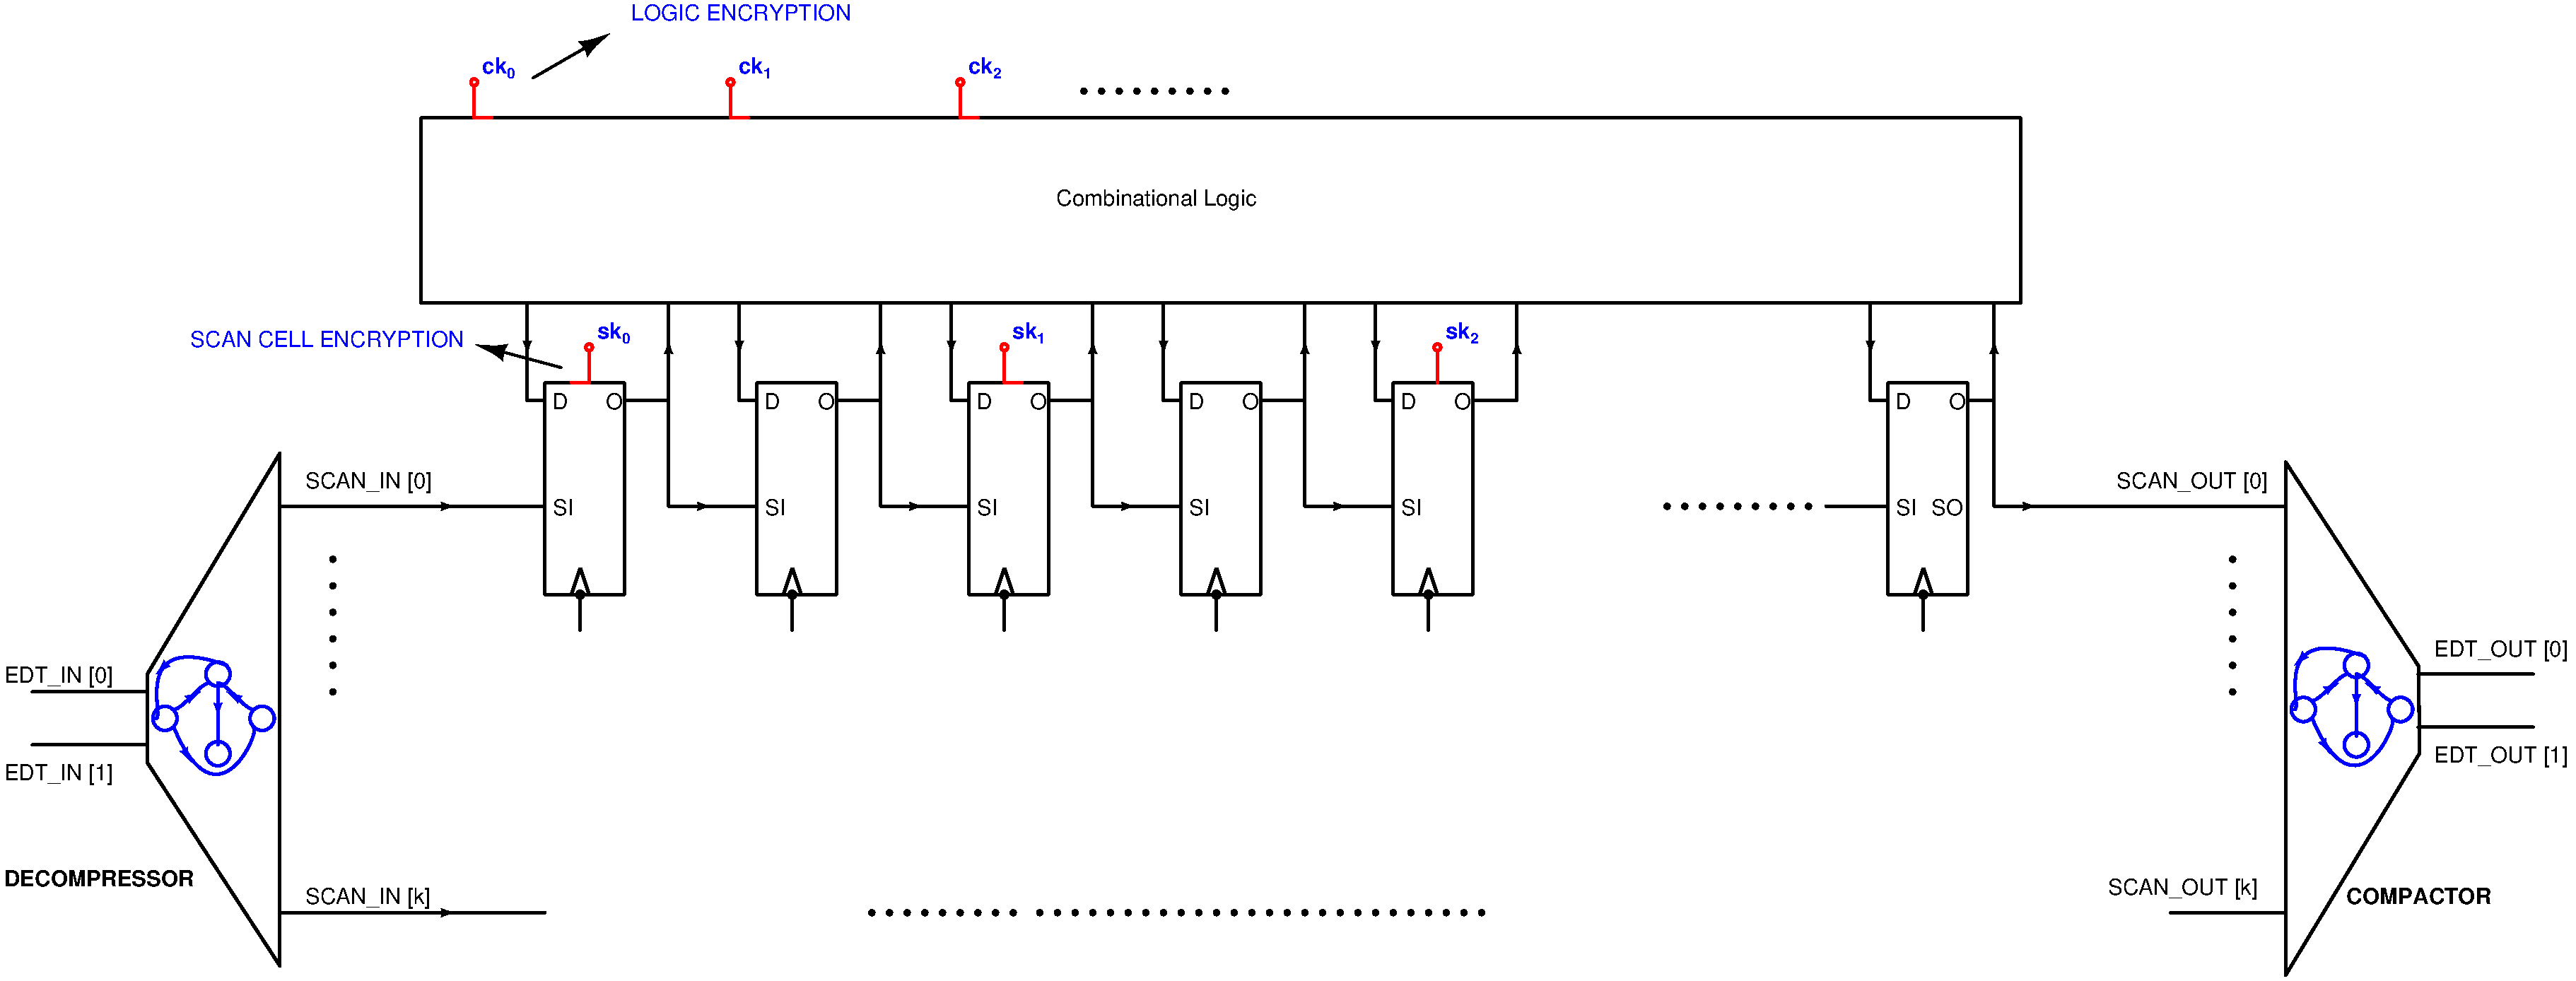
\includegraphics[scale=0.2]{fig/encrypted-DFT.pdf}
\end{center}
\end{figure}
\end{frame}

\begin{frame}{Libary Scan Cell}
\begin{figure}
\begin{center}
\label{fig:sc}
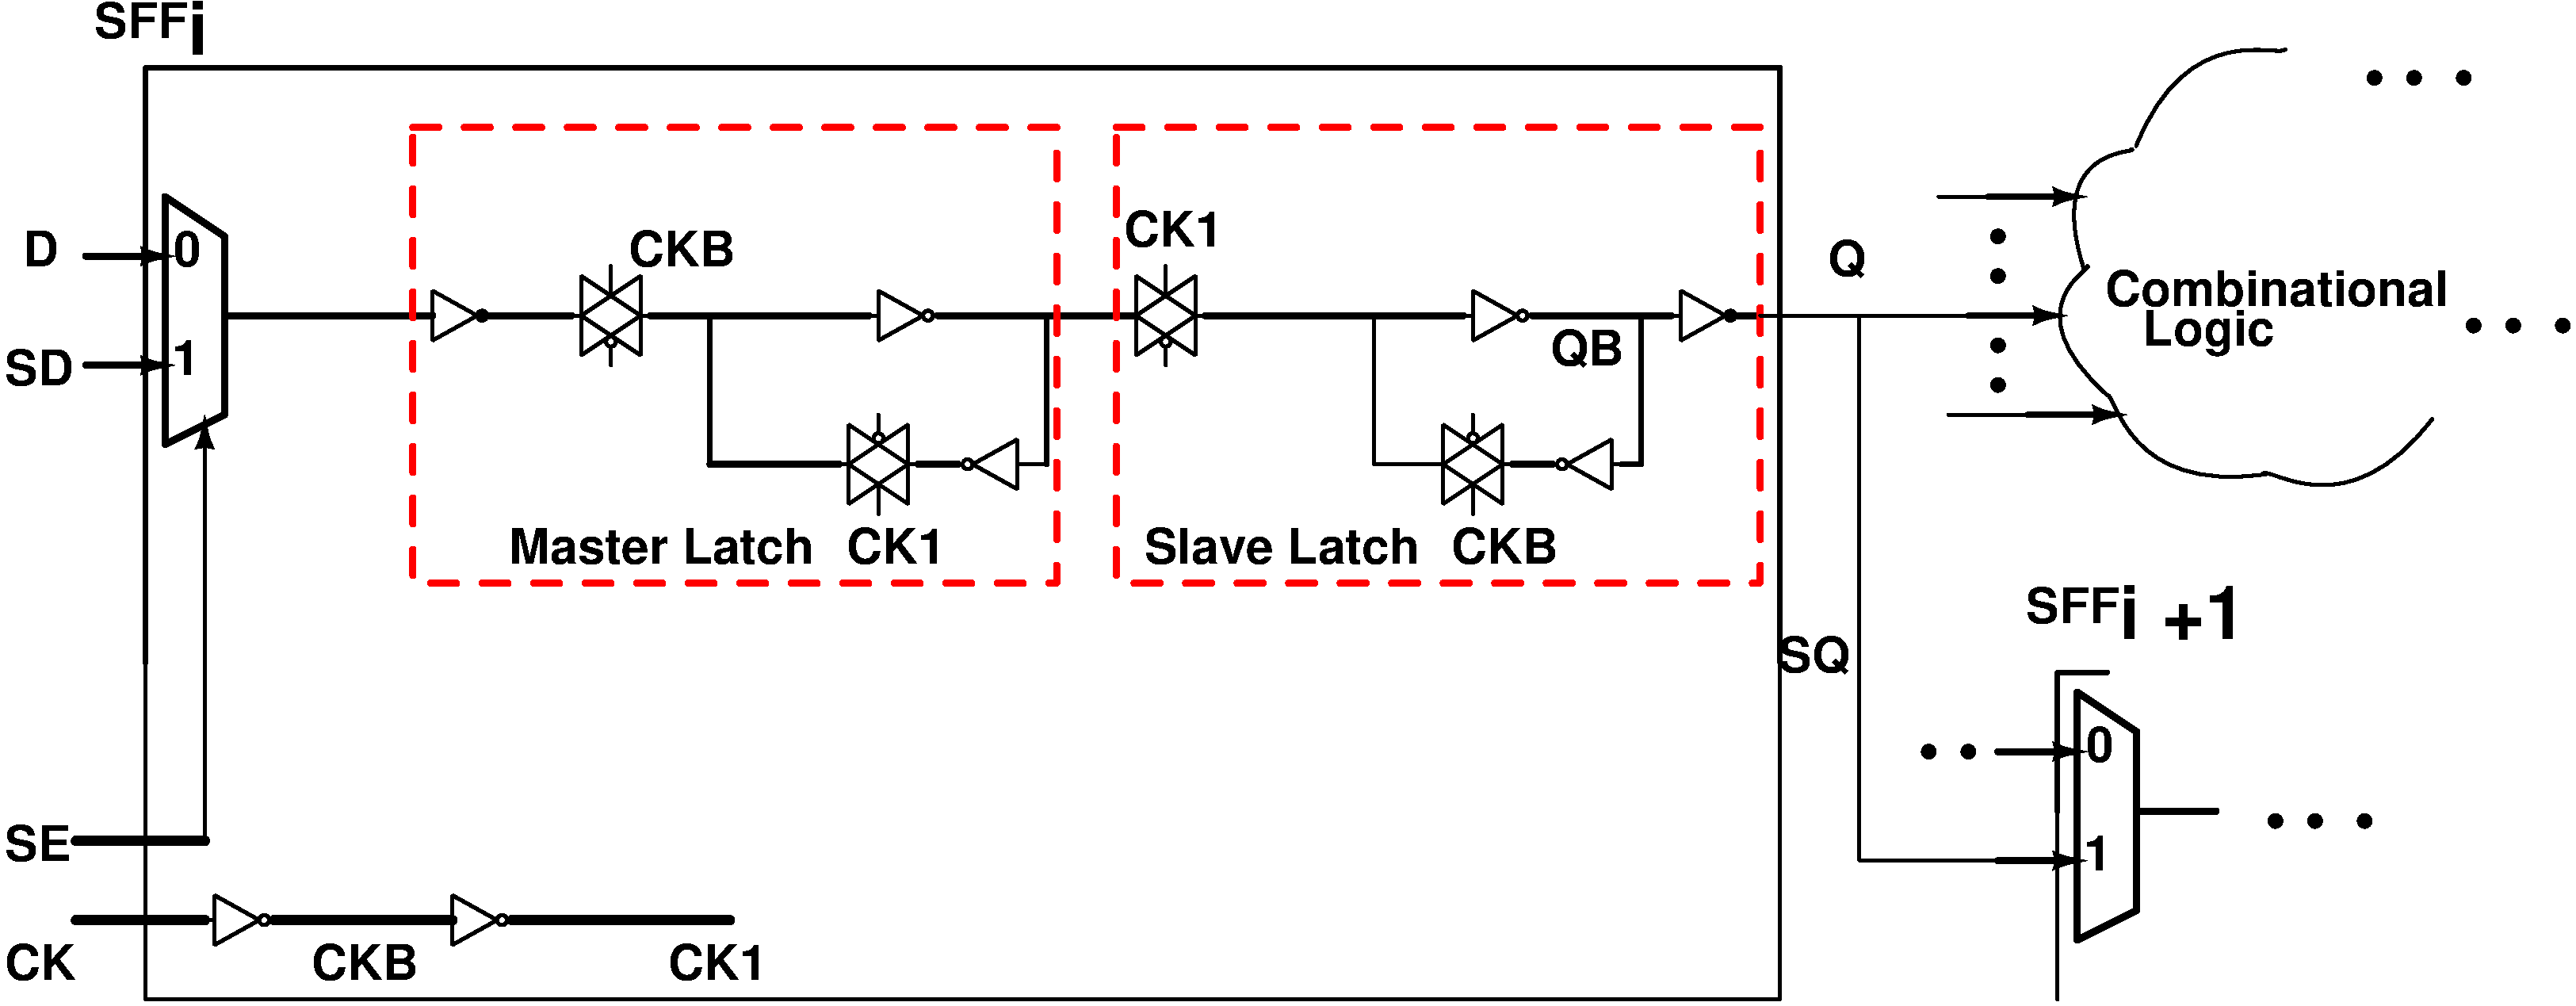
\includegraphics[scale=0.2]{fig/traditional-scanflop.pdf}
\end{center}
\end{figure}
\end{frame}

\begin{frame}{Existing Encrypted Scan Cell}
\begin{figure}
\begin{center}
\label{fig:encrypted-sc}
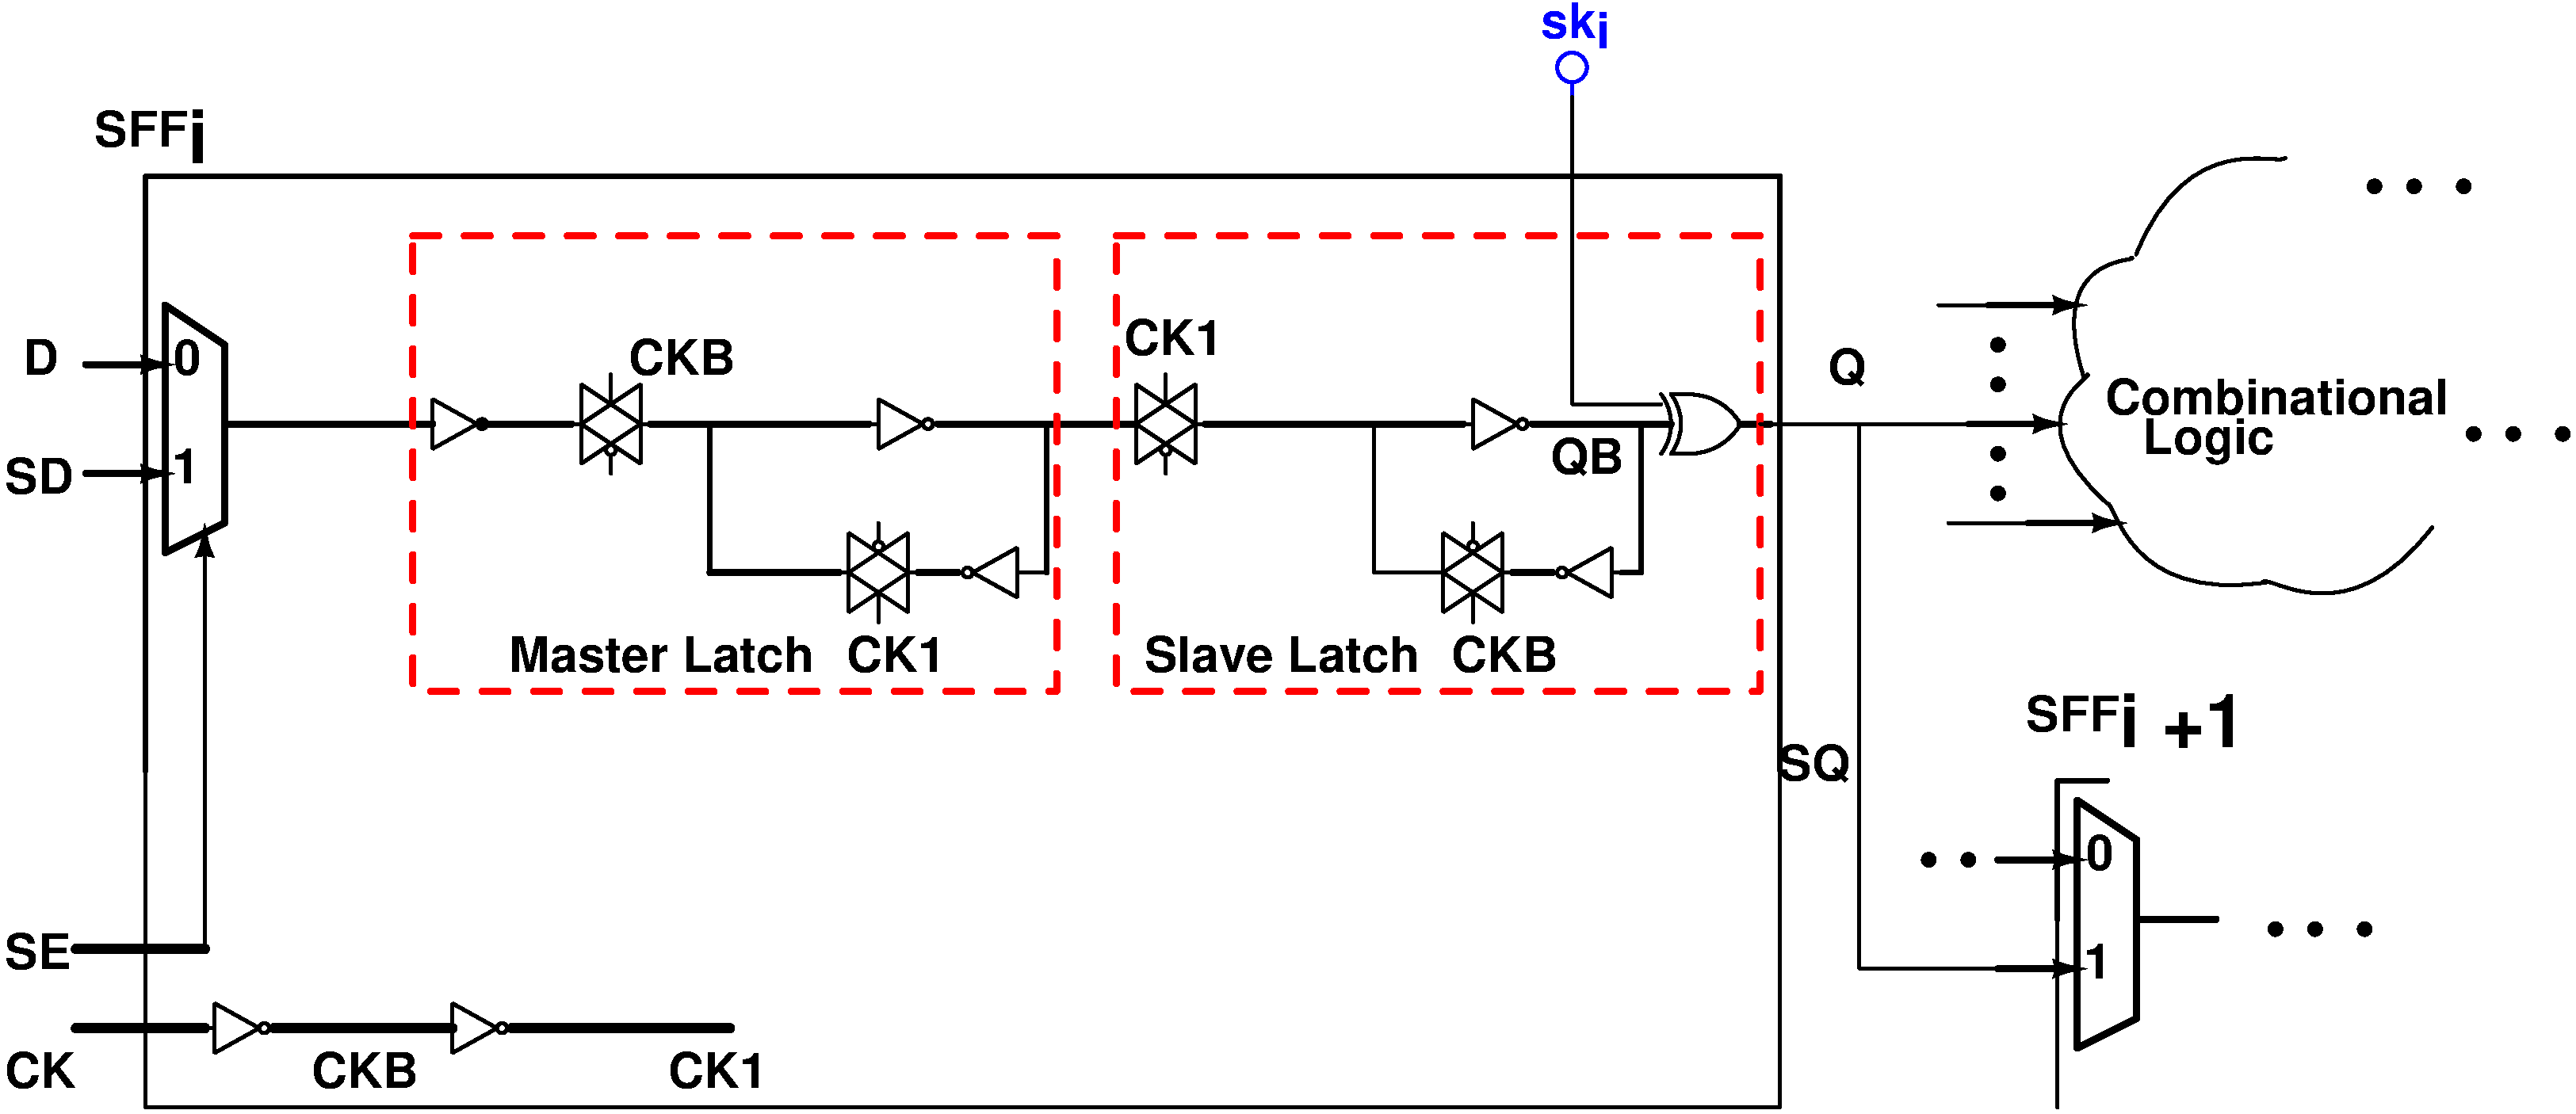
\includegraphics[scale=0.2]{fig/encrypted-scanflop.pdf}
\caption{It is possible to decrypt the correct key\footnote{L. Alrahis, "ScanSAT: Unlocking Obfuscated Scan Chains", ASP-DAC 2019}}
\end{center}
\end{figure}
\end{frame}

\begin{frame}{Proposed Encrypted Scan Cell}
\begin{figure}
\begin{center}
\label{fig:encrypted-sc}
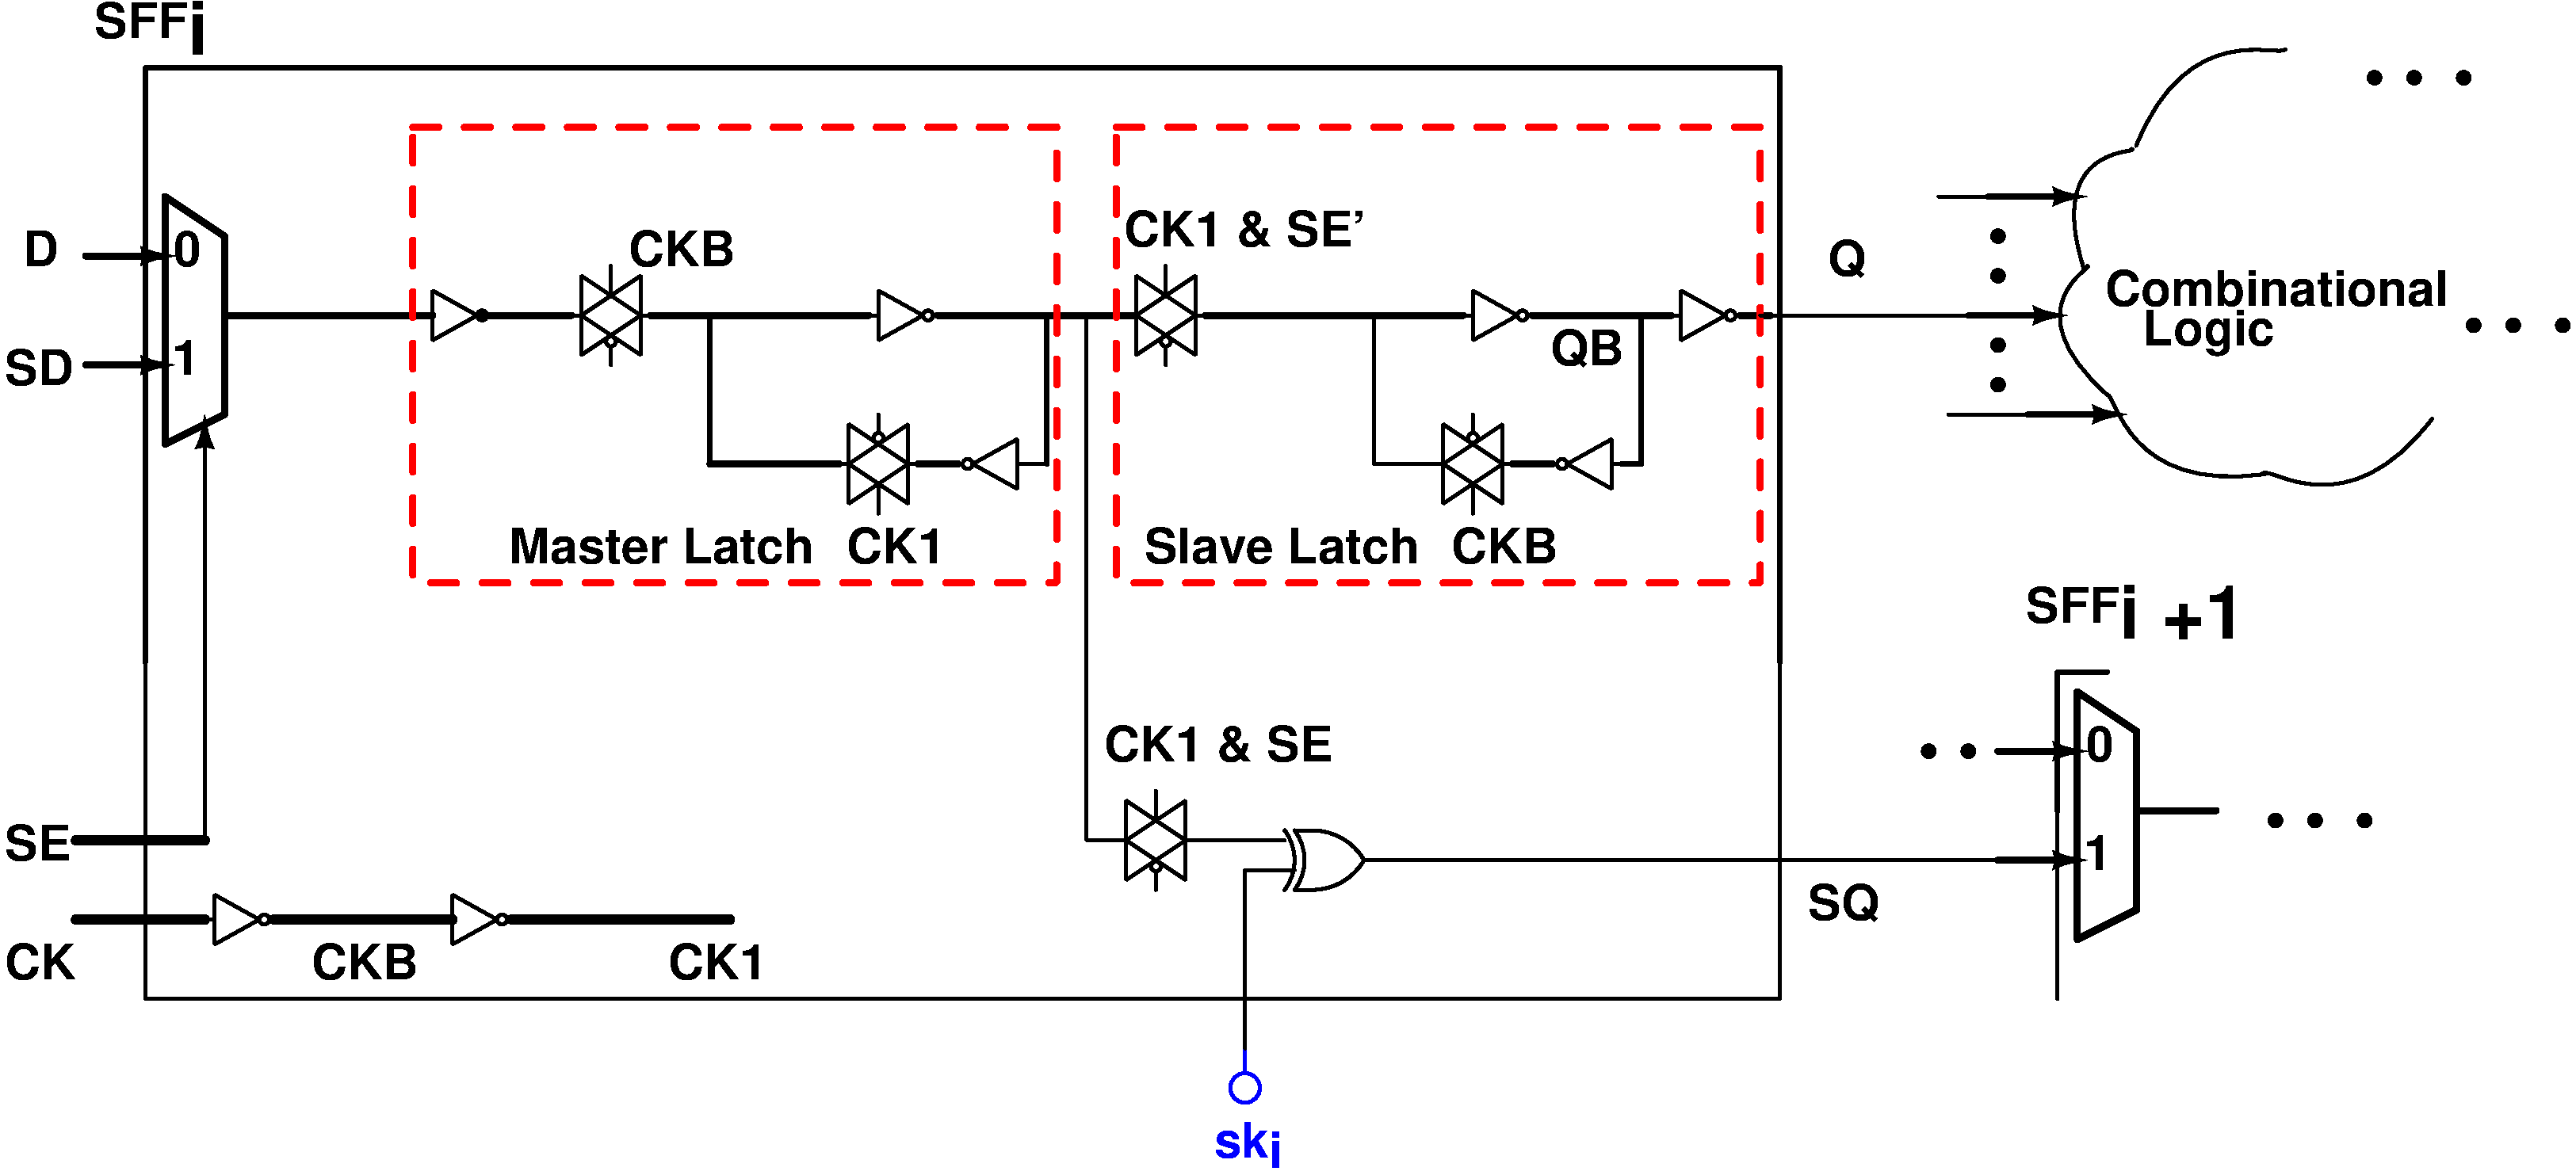
\includegraphics[scale=0.2]{fig/encrypted-scanflop-2.pdf}
\caption{Only combinational portion of the sequential key locks the functional mode of operation}
\end{center}
\end{figure}
\end{frame}


\begin{frame}{SAT attack on Encrypted DFT (BYPASS mode)}
\begin{itemize}
	\item All the scan chains connect together to form 1 single chain
	\item The scan cells can be removed and their inputs/outputs can be unrolled as a function of the XOR gates along the scan-shift path
\end{itemize}
\end{frame}

%\begin{frame}{SAT attack on Encrypted DFT (BYPASS mode)}
%\begin{figure}
%\begin{center}
%\caption{Scan-unrolled circuit }
%\label{fig:encrypted-sc}
%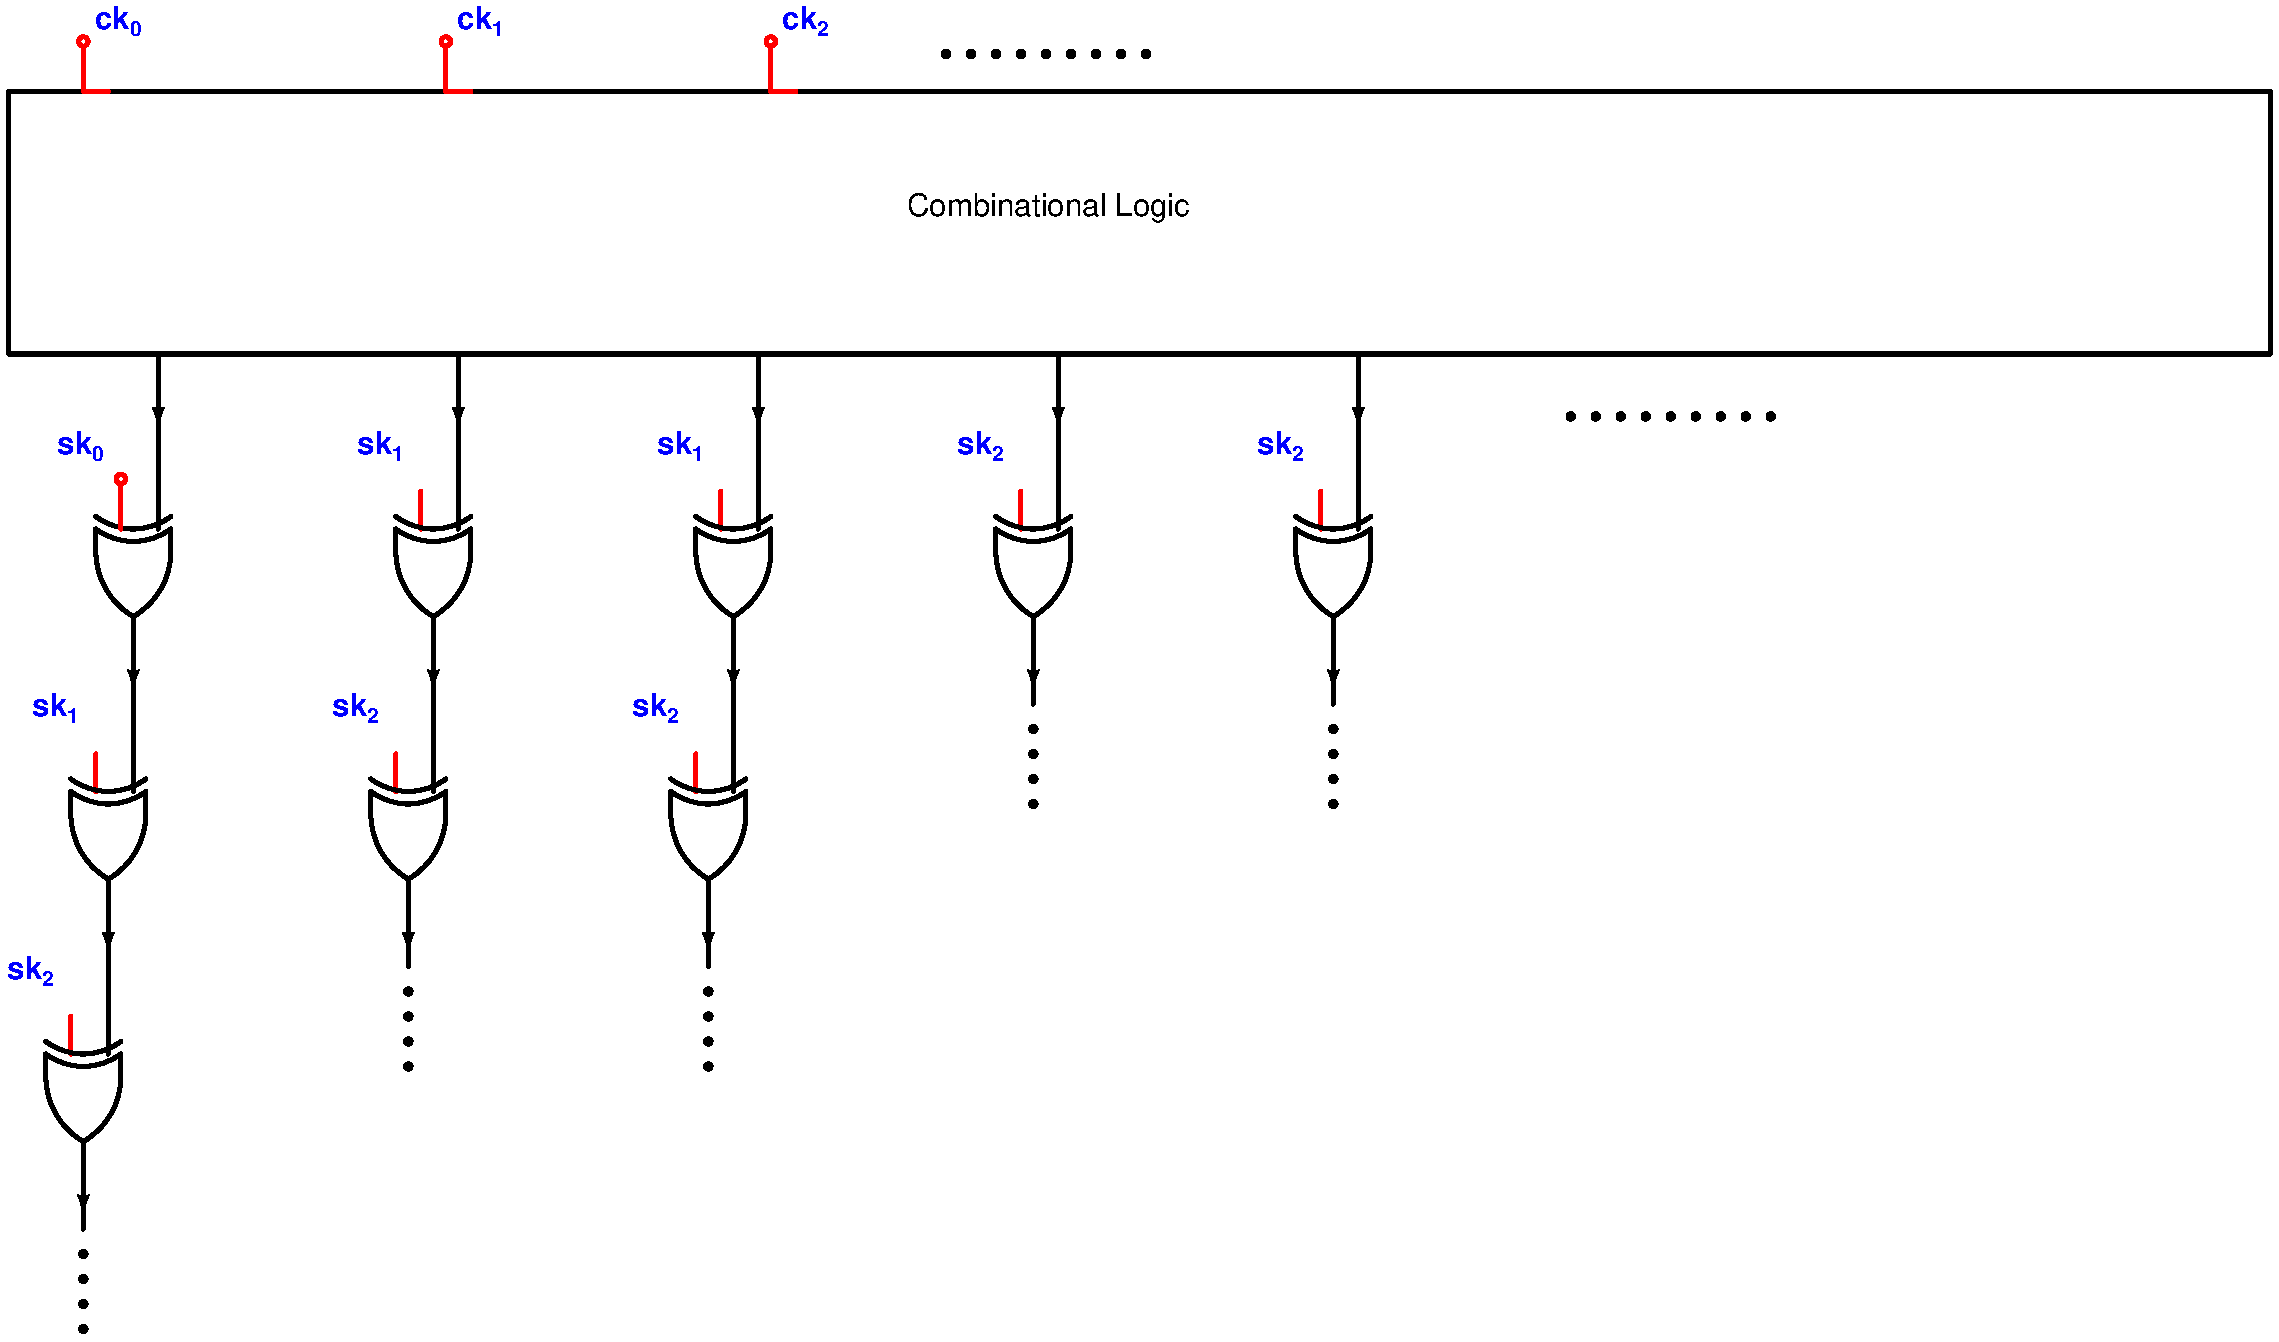
\includegraphics[scale=0.2]{fig/SATattack-on-encrypted-DFT.pdf}
%\end{center}
%\end{figure}
%\end{frame}

\begin{frame}{Example}
\begin{figure}
\begin{center}
\caption{s27 circuit with all scan cells encrypted}
\label{fig:s27}
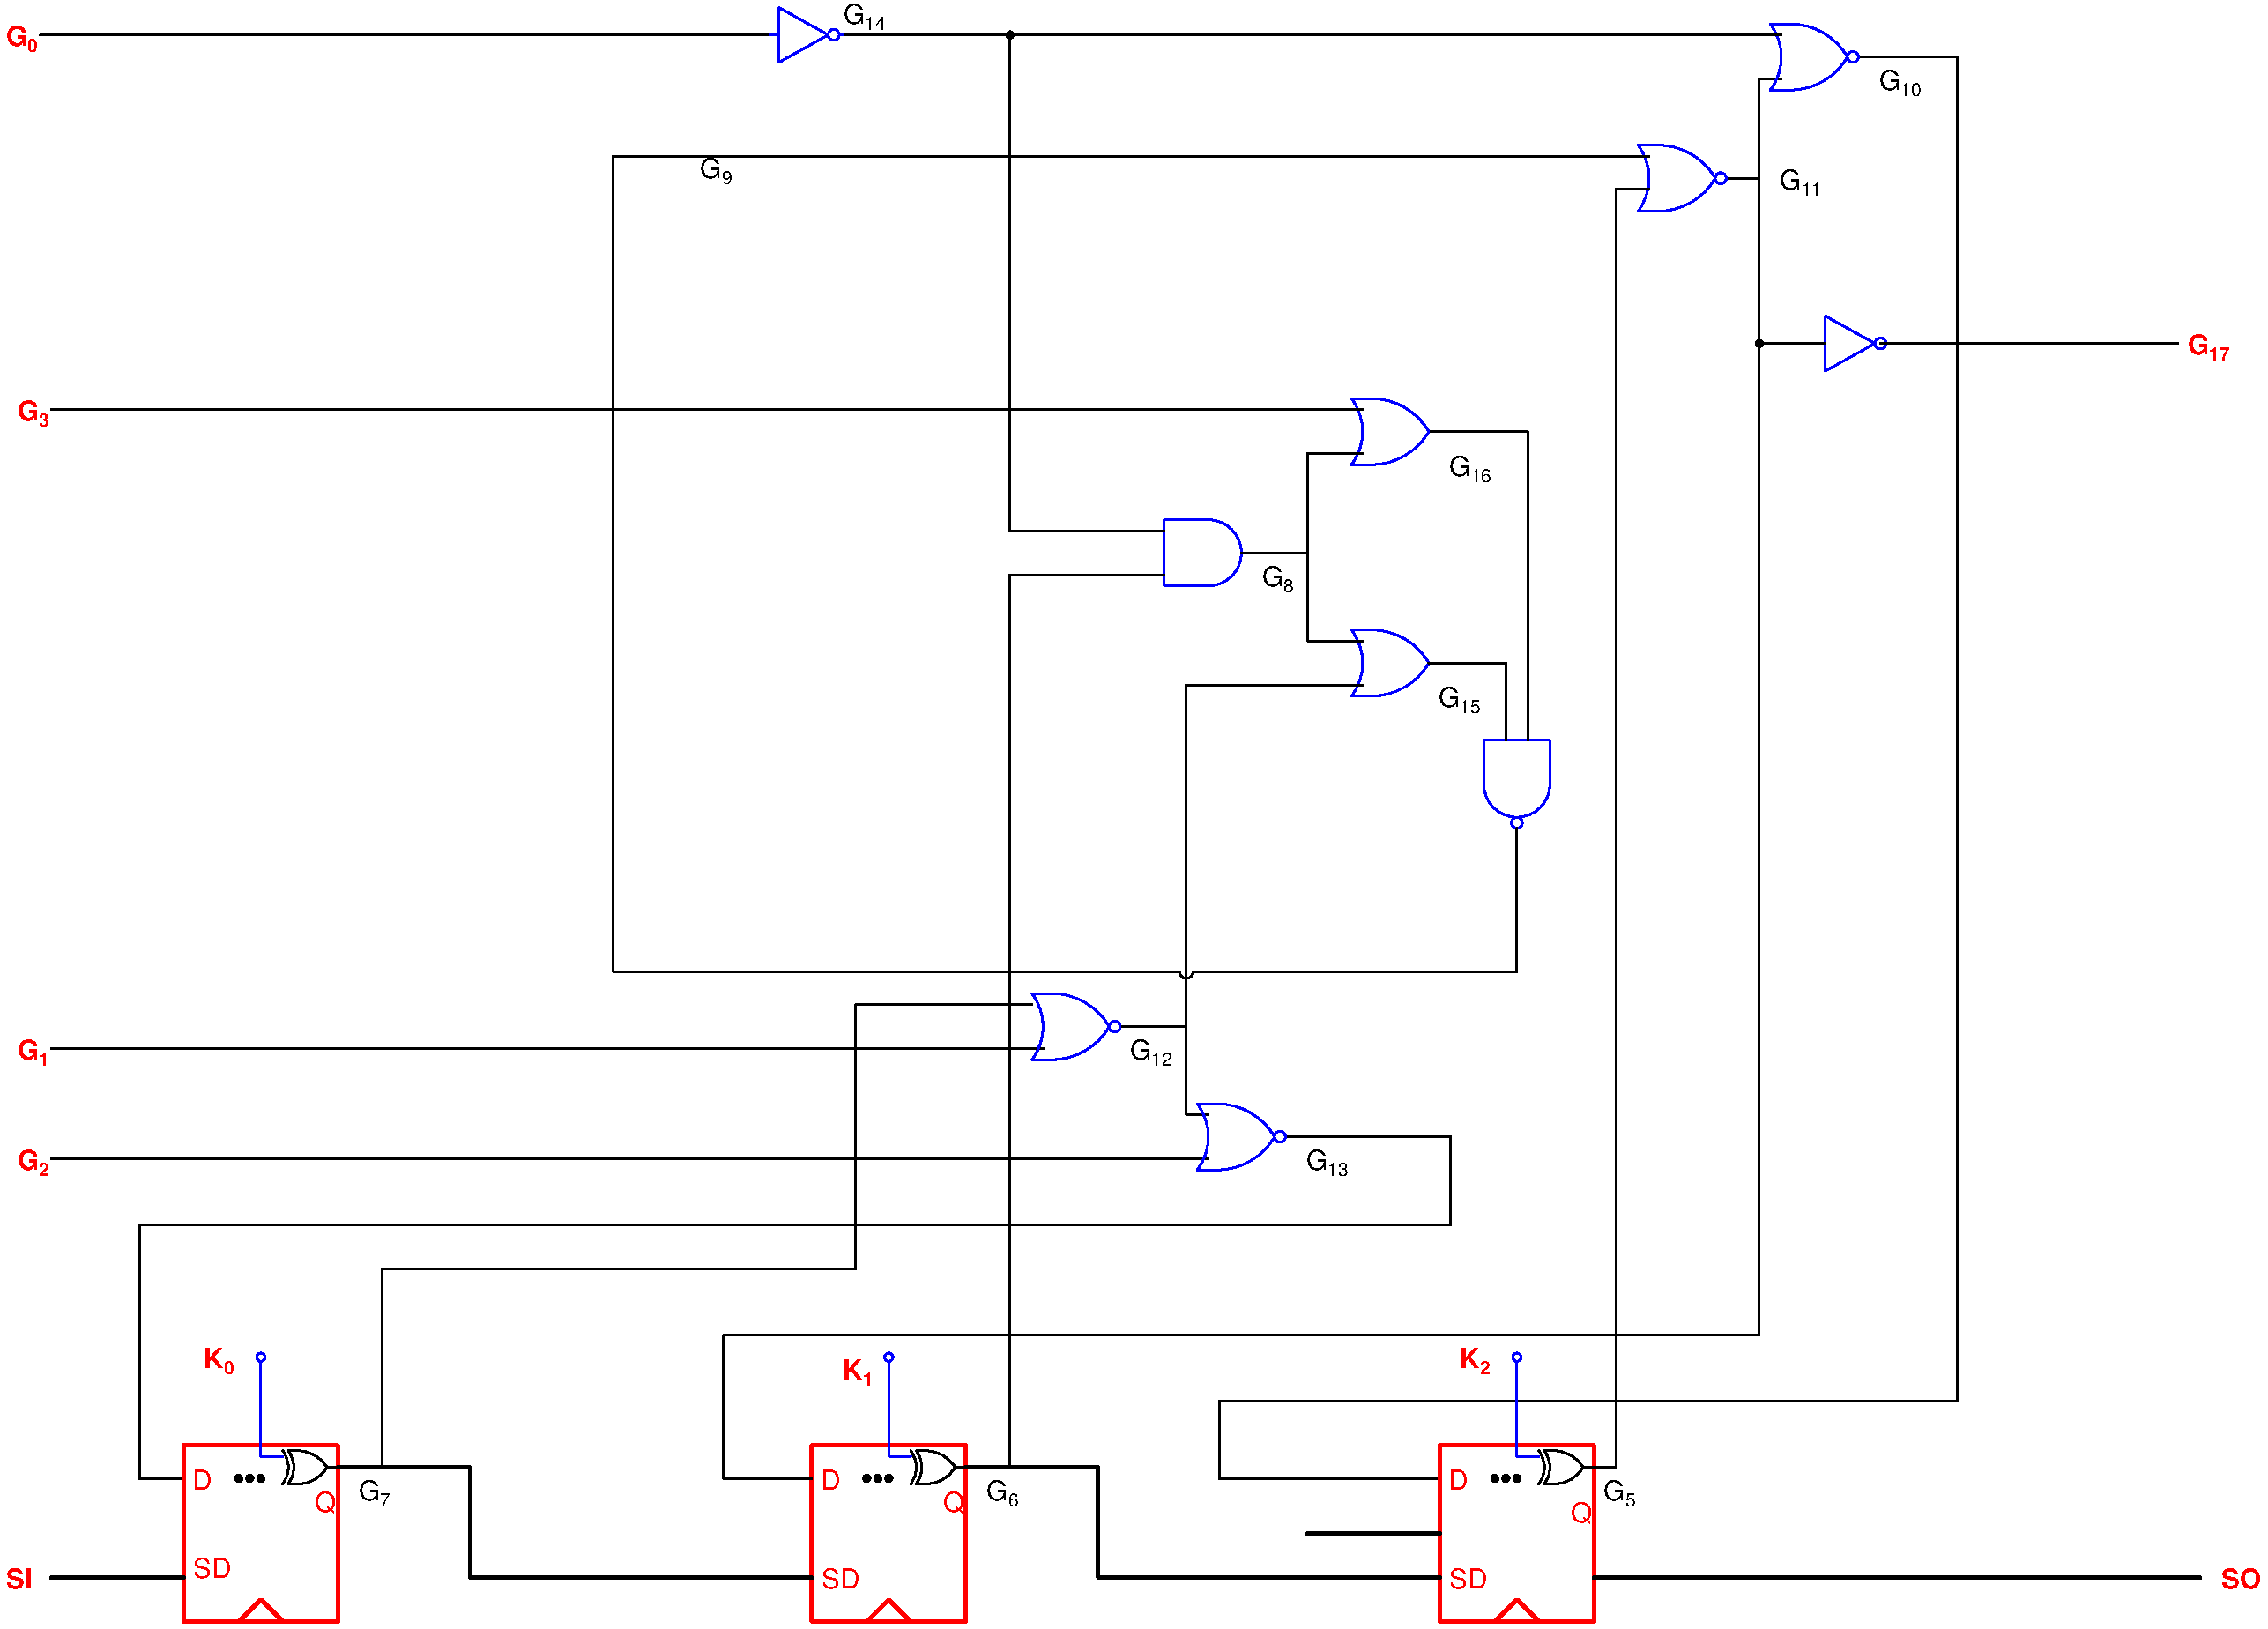
\includegraphics[scale=0.15]{fig/s27.pdf}
\end{center}
\end{figure}
\end{frame}

\begin{frame}{Example}
\begin{figure}
\begin{center}
\caption{s27 circuit after scan unroll}
\label{fig:s27-after-scan-unroll}
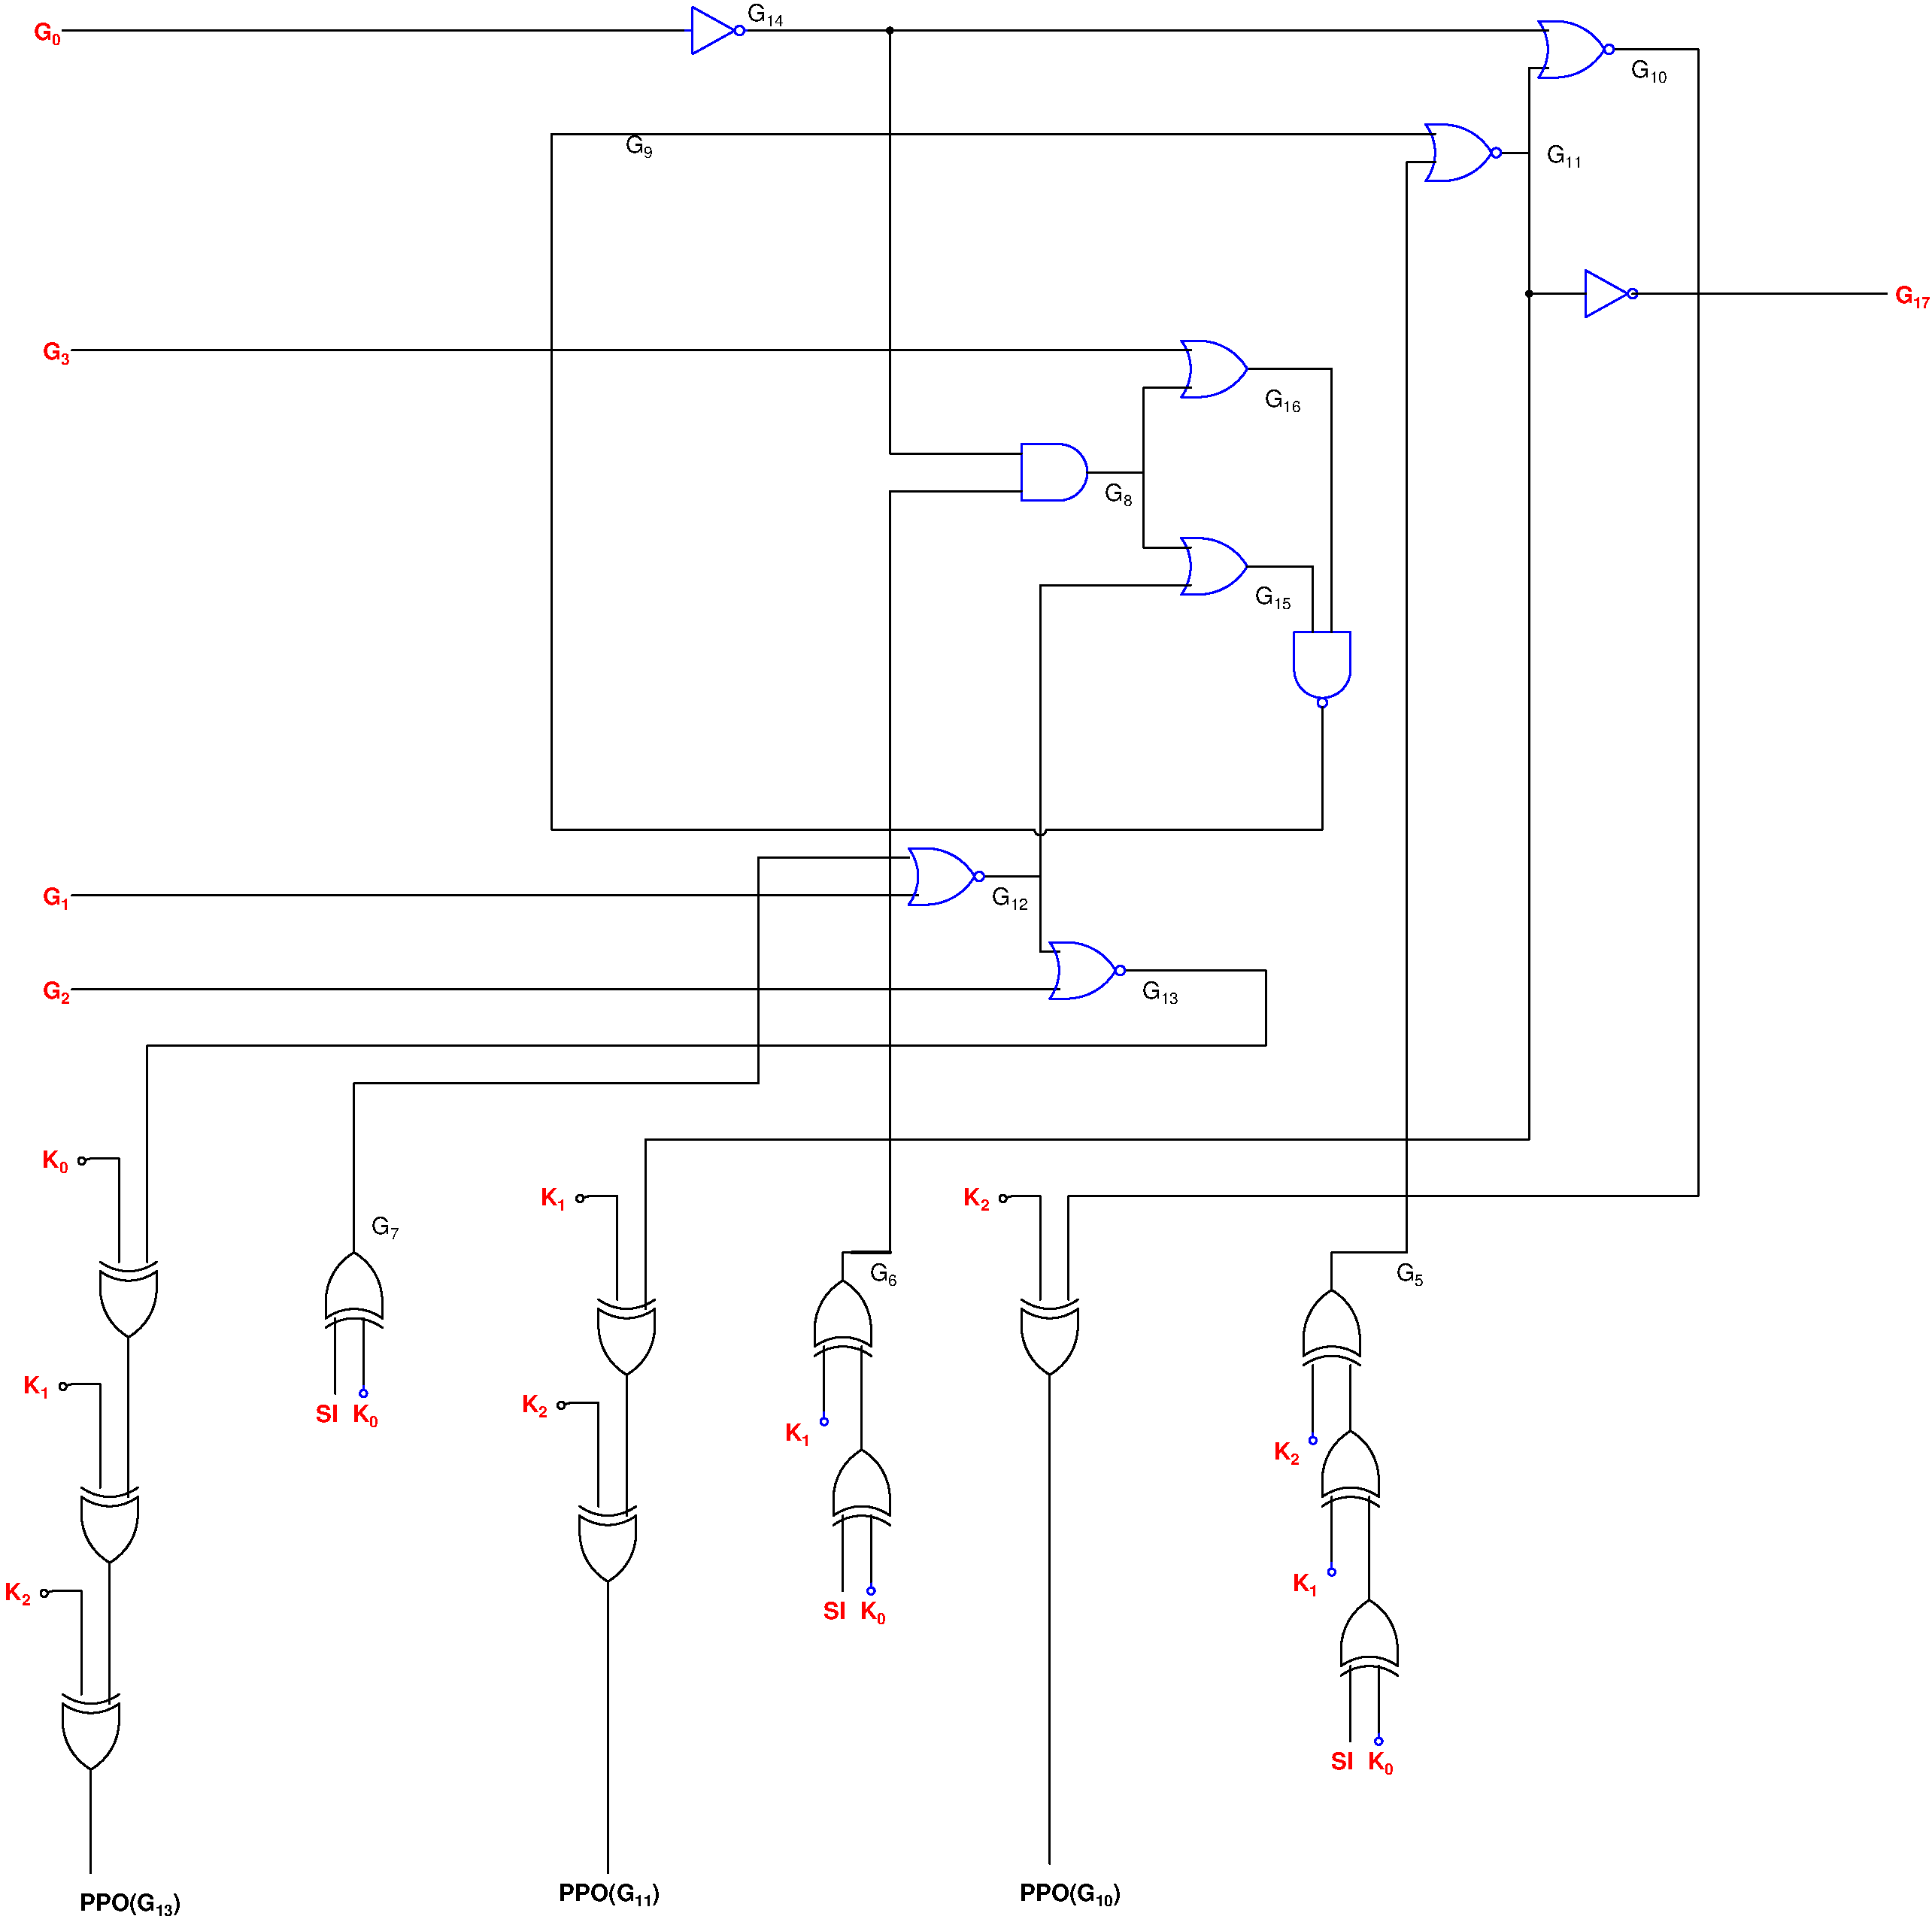
\includegraphics[scale=0.12]{fig/s27_after_scanunroll.pdf}
\end{center}
\end{figure}
\end{frame}

\begin{frame}{Example}
\begin{figure}
\begin{center}
\caption{s27 circuit after scan unroll - SAT overhead}
\label{fig:s27-after-scan-unroll-SAT-overhead}
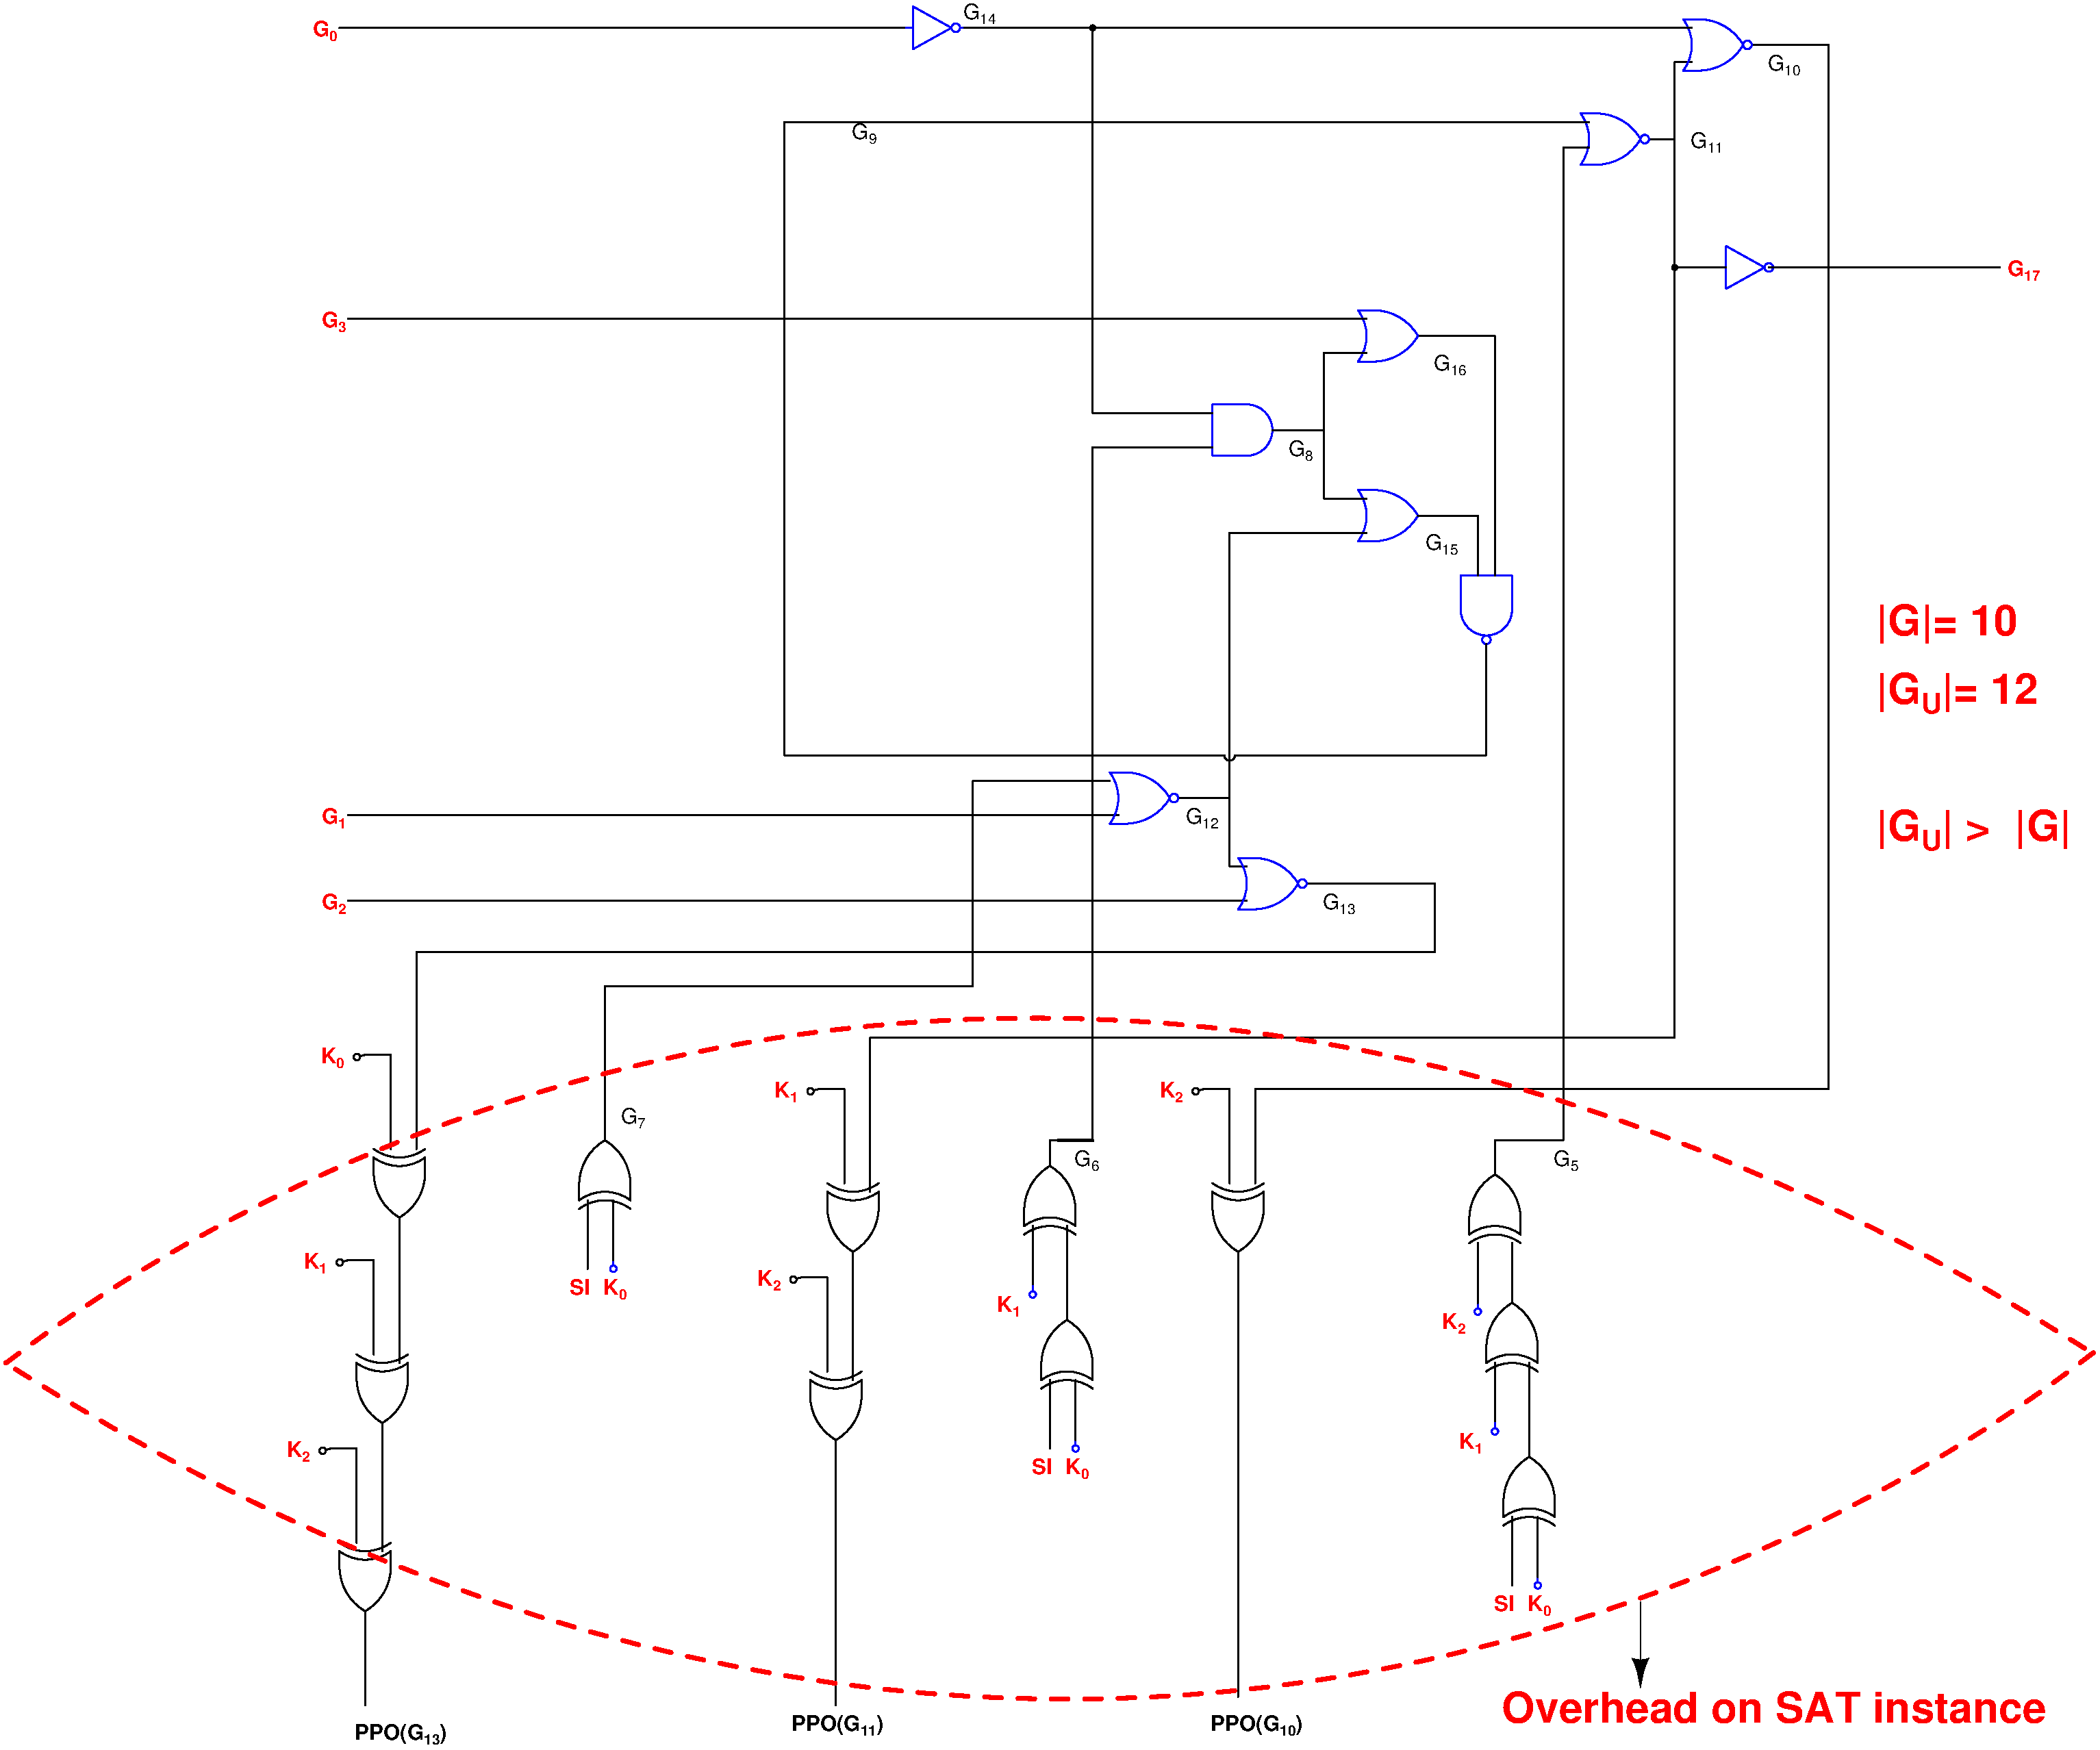
\includegraphics[scale=0.12]{fig/s27_after_scanunroll_SAToverhead.pdf}
\end{center}
\end{figure}
\end{frame}

